\documentclass{article}

\usepackage{fancyhdr}
\usepackage{ragged2e}
\usepackage{graphicx}
\usepackage{caption}
\usepackage{geometry}
\usepackage{amsmath}
\usepackage{rotating}

\usepackage{listings}
\usepackage{color}

\definecolor{dkgreen}{rgb}{0,0.6,0}
\definecolor{gray}{rgb}{0.5,0.5,0.5}
\definecolor{mauve}{rgb}{0.58,0,0.82}

\lstset{frame=tb,
  language=Java,
  aboveskip=3mm,
  belowskip=3mm,
  showstringspaces=false,
  columns=flexible,
  basicstyle={\small\ttfamily},
  numbers=none,
  numberstyle=\tiny\color{gray},
  keywordstyle=\color{blue},
  commentstyle=\color{dkgreen},
  stringstyle=\color{mauve},
  breaklines=true,
  breakatwhitespace=true,
  tabsize=4
}

\setcounter{secnumdepth}{1}

\usepackage{chngcntr}
\counterwithin{figure}{section}

\renewcommand*{\thepage}{C\arabic{page}}

\pagestyle{fancy}
\lhead{ACME Robotics}
\chead{\#8367}
\rhead{\ifcontents Contents \else Week \thesection \fi}

\newif\ifcontents
\contentstrue

\makeatletter
\renewcommand{\@seccntformat}[1]{}
\makeatother

\begin{document}\contentsfalse

\subsection{Print the Marker}
%! Give Kelly the marker CAD to be printed
This week Ben finished revising the model of the team marker in Inventor Pro 2018. He then converted the .iam file to an .stl file to be printed. Then, he gave Kelly the file to be printed. Towards the end of the meeting, Ben tapped about 10 churros to be used in the drive train. Figure \ref{fig:marker} shows the final marker. 

\begin{figure}
    \centering
    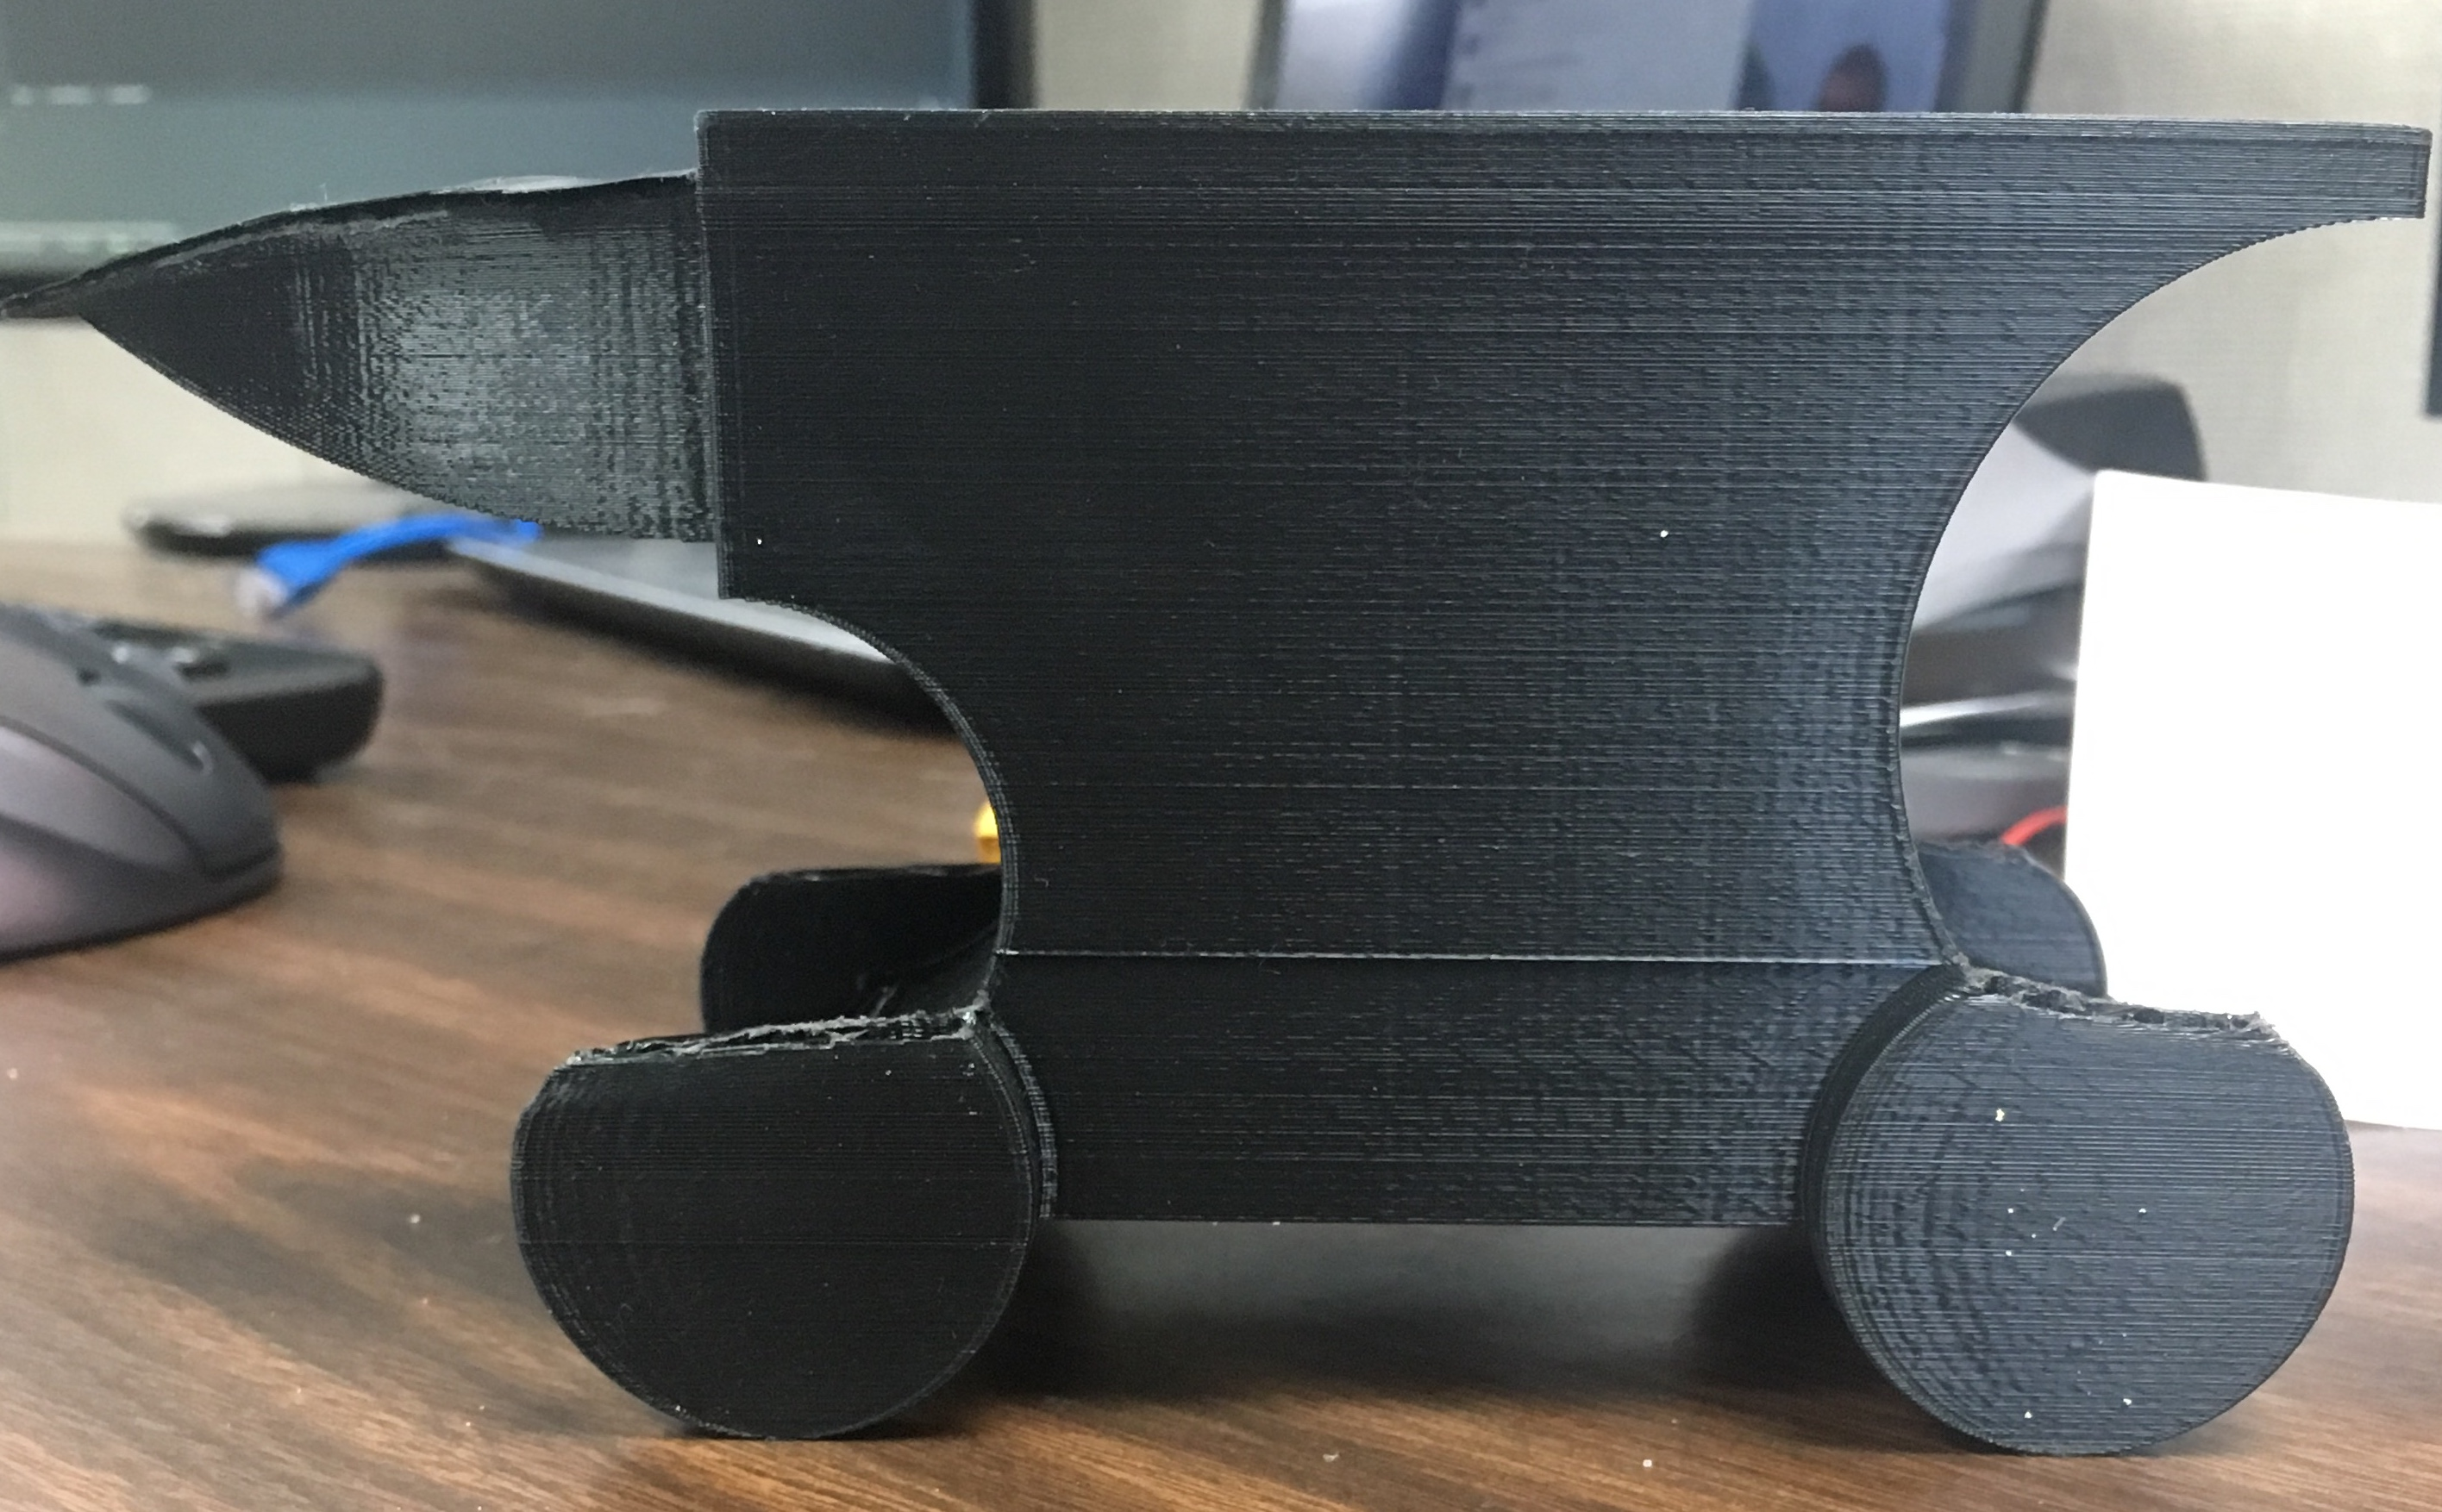
\includegraphics[width=.6 \textwidth]{09_10-29/images/anvil_marker.jpg}
    \caption{Anvil Marker}
    \label{fig:marker}
\end{figure}

\subsection{Fabrication}
%! Start to fabricate the parts for the robot.
Now that the team had most of the parts of the robot, they could begin fabricating the robot. To assemble the intake and drivetrain, the metal cross beams and Vex rollers needed to be cut down to size. Jon had a chop saw and band saw at his house so he took the Vex rollers and cross beams home to be cut. To complete the rollers for the intake, holes had to be drilled in the rollers for the surgical tubing. After drilling a test piece, Jon had to rearrange the way the rollers were clamped in the vice. He then drilled the rest of the Vex rollers.
\subsection{Lift Fabrication}
%! Lift bearing blocks 
Oren went to GSS a sponsoring company to work with a one of there mechanical engineer, on milling custom bearing blocks for the lift. The team this year wanted to custom fabricated a lift that would be robust enough to hold and lift the in both the the beginning and end of the match. 

\end{document}